\documentclass[12pt,a4paper]{article} % A4 paper and 11pt font size


\usepackage[utf8x]{inputenc}
\usepackage{braket}
\usepackage{amsmath}
\usepackage{amssymb}
\usepackage{bm}
%\usepackage[utf8]{inputenc}
\usepackage{verbatim}
\usepackage{tikz}
%\usepackage{tikz-feynman}
%\usepackage{pgfornament}
\usepackage{pgfplots}
\usepackage{pgffor}
\usepackage[version-1-compatibility]{siunitx}
\usepackage{fancyhdr}
\usepackage{lipsum}
\usepackage{gensymb}
\usepackage{framed}
\usepackage{cancel}
\usepackage{slashed}
\usepackage{hyperref}
\usepackage{pdflscape}
\usepackage{graphicx}
\usepackage{caption}
\usepackage{subcaption}
\usepackage{geometry}
\usepackage{yfonts}
\usepackage{calc}
\usepackage{cite}

\setlength{\parindent}{2em}
\setlength{\parskip}{1em}
\newcommand{\goth}[1]{{\Huge\textfrak{#1}}}
\renewcommand{\baselinestretch}{1.1}

\newcommand{\br}{\mathcal{B}}
\newcommand{\tmg}{\tau\to\mu\gamma}
\newcommand{\tlg}{\tau\to\ell\gamma}
\newcommand{\htm}{h\to \tau \mu}

 \geometry{
 a4paper,
 total={210mm,297mm},
 left=28mm,
 right=28mm,
 top=30mm,
 bottom=40mm,
 }


%----------------------------------------------------------------------------------------
%	TITLE SECTION
%----------------------------------------------------------------------------------------
%\setlength\parindent{0pt} % Removes all indentation from paragraphs - comment this line for an assignment with lots of text


\pagenumbering{arabic}
\begin{document}
\pagestyle{empty}

\newcommand{\HRule}{\rule{\linewidth}{0.5mm}}

\begin{titlepage}

    \begin{center}
        %\textsc{\large SN: 587623}
        \vspace*{5cm}

        %\pgfornament[width = 0.9\textwidth, symmetry=v]{88}\\[0.75cm]
        \HRule \\[0.75cm]
        \huge \textbf{Thesis} \\[0.5cm]
		\Huge \textbf{A search for $\bm{\tau\to\ell \gamma}$ \\at Belle and Belle II}\\[0.5cm]
        %\pgfornament[width = 0.9\linewidth]{88}\\[1.5cm]
        \HRule \\[1.5cm]
        \begin{minipage}{0.4\textwidth}
        \begin{center}

        \large By \\[0.75cm]
        \huge Braden \scshape Moore \\[0.5cm]
        \normalsize \normalfont Master of Science \\
        The University of Melbourne \\

        \end{center}
        \end{minipage}

        \vfill

        \large \today
    \end{center}


\newpage
\end{titlepage}
%----------------------------------------------------------------------------------------
\pagestyle{empty}
\tableofcontents
\newpage

\pagestyle{fancy}
\pagenumbering{arabic}
\rhead{\textsc{Thesis: $\tlg$}}
\setcounter{page}{1}


\section{Literature Review}

\subsection{Introduction}

Lepton flavour violation (LFV) is an exciting field of research at the frontier of particle physics. Searches for LFV can probe a wide variety of new physics (NP) scenarios. We will not be looking at all LFV; in this literature review we specifically cover charged LFV of the form $\tlg$. Of the tau processes, these modes are predicted to be the most sensitive to NP. We choose to investigate tau LFV rather than, say, muon LFV, for two main reasons. Firstly, the tau processes have predicted branching fractions of $\sim 5 - 6$ orders of magnitude greater than the analogous muon processes, due to the differences in mass \cite{Paradisi:2016}. The decay $\tmg$ has a predicted branching fraction $\sim 6$ orders of magnitude greater than the analogous $\mu\to e \gamma$! Secondly, if this NP introduces Higgs-like particles, we would observe the NP more strongly in the tau sector, since taus couple more strongly to Higgs than do muons.


\begin{figure}[h]
\centering
%\includegraphics[width=0.6\textwidth]{images/taumugamma.png}
\caption{Diagram of $\tmg$ in the Standard Model}
\label{}
\end{figure}

\subsection{LFV and the Standard Model}

LFV necessarily requires generation mixing between leptons to occur. Though this is prohibited in the Standard Model, the discovery of neutrino oscillations proves that flavour mixing does occur in our universe; that is, flavour is not conserved. We seek to discover whether this LFV can be observed in other areas of flavour physics.

In the Standard Model + massive neutrinos, the only source of LFV is from the operators responsible for neutrino mass. However, the relevant Feynman diagrams (see Figure) are ``loop suppressed'' and proportional to the GIM factor, given as $\left(\frac{m_\nu}{M_W}\right)^4$; as neutrino mass is very small ($\mathcal{O}(\SI{0.3}{eV})$) we expect the LFV effects to be negligible! With these operators the branching ratio for, say, $\tmg$ is $\sim 10^{-40}$ \cite{Passemar:2015}. With such little SM background, observation of an LFV process of the type $\tlg$ would be an unambiguous signature of NP.

\subsection{Other LFV}

In many NP models, LFV is not limited to just $\tlg$ decays. There have been searches for other LFV modes, such as $\mu\to e \gamma$, and $\tau\to 3\ell$. Current limits on the branching fractions are given in Figure \ref{tab:current lfv bounds} below \cite{Paradisi:2016}.

\begin{figure}[h]
\centering
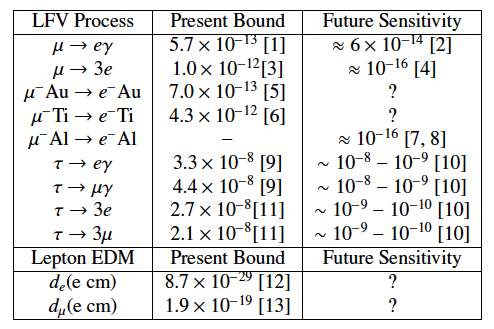
\includegraphics[width=0.6\textwidth]{images/lfv-bounds.png}
\caption{Current experimental limits on various LFV processes (Paradisi, 2016)}
\label{tab:current lfv bounds}
\end{figure}

Moving into future sensitivities accessible from experiments such as Belle II, we see that the upper limits of branching fractions for $\tlg$ decays could be improved by $1-2$ whole orders of magnitude!

\subsection{Hints of LFV beyond the Standard Model}

Motivations behind the search for LFV come from both theoretical and experimental results. Chief amongst the experimental motivations is the existence of neutrino mixing, though anomalous results such as the $\htm$ excess observed at CMS in 2015 also hint at LFV beyond the Standard Model. On the theoretical side, LFV is predicted in a variety of NP models. In fact, many models which introduce mechanisms to generate neutrino mass also inadvertantly allow LFV in other sectors of non-negligible order! We shall discuss these motivations below.


\subsubsection{Neutrino mixing}

The discovery that flavour mixing can occur in the neutrino sector \cite{SuperK:1998}\cite{SNO:2002} proves that neutrinos have mass. Both the concept of massive neutrinos, and by extension the mechanisms which generate neutrino mass, are not predicted or explained by the SM. This tells us that the lepton sector is not fully understood.

There are many NP models which introduce mechanisms to give neutrinos mass. These include SUSY, seesaw models, and many others. In introducing these mechanisms, many of these models inadvertently introduce LFV! As a particle example, a Type-II seesaw model posits a scalar triplet of Higgs-like particles \cite{Passemar:2015}. This triplet comprises a doubly-charged Higgs, a singly-charged Higgs, and a neutral Higgs. As show in Figure X below, lepton-flavour violating processes could proceed via leptons coupling to these scalars!


\begin{figure}[h]
\centering
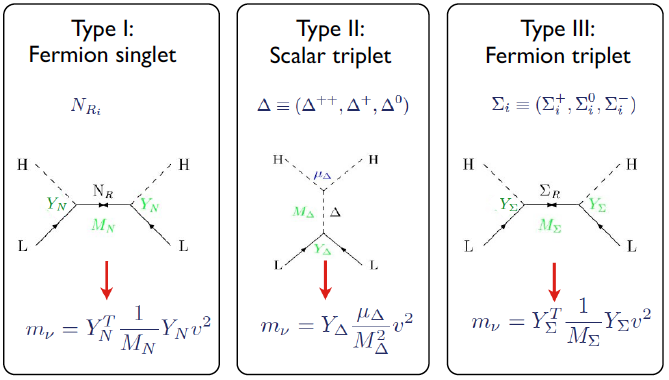
\includegraphics[width=0.7\textwidth]{images/seesaw.png}
\caption{New particles introduced in seesaw models (Passemar, 2015)}
\label{}
\end{figure}

\begin{figure}[h]
\centering
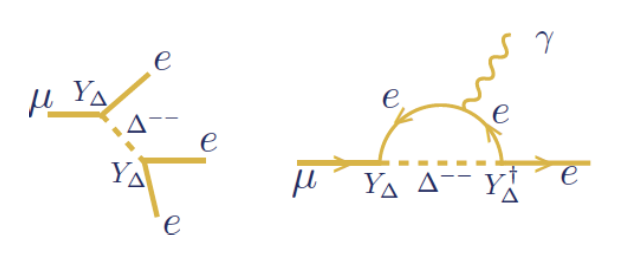
\includegraphics[width=0.5\textwidth]{images/seesaw-lfv-modes.png}
\caption{Scalars introduced in Type-II seesaw models mediating LFV decays (Passemar, 2015)}
\label{}
\end{figure}




\subsubsection{$\htm$ excess}

Hints of LFV can come in the form of experimental results which are not consistent with the SM. One such ``anomaly’’ is the $\htm$ excess. In 2015, CMS found a $2.4\sigma$ excess in the branching fraction of $\htm$ \cite{CMS:2015a}. This process is lepton flavour violating, so in the SM its branching fraction is expected to be consistent with zero. However it was determined

\begin{equation}
\br(h\to \tau \mu) = (0.84^{+0.39}_{-0.37})\%
\end{equation}


Also in 2015 was a similar search performed by ATLAS \cite{ATLAS:2015}, in which an excess of $1.2\sigma$ was found in the $\htm$ decay. 

\begin{equation}
B(\htm) = (0.77 \pm 0.66)\%
\end{equation}

Though this $1.2\sigma$ result is less indicative of NP, it still provides hints as to where NP could occur. These results indicate possible new physics in the Higgs sector! Several models, including Two-Higgs Doublet Models (2HDM), introduce new Higgs-like particles; these particles can couple with leptons to allow lepton flavour violating processes \cite{Harnik:2012}. In fact, LFV can occur naturally in any model with more than one Higgs doublet.


\begin{figure}[h]
\centering
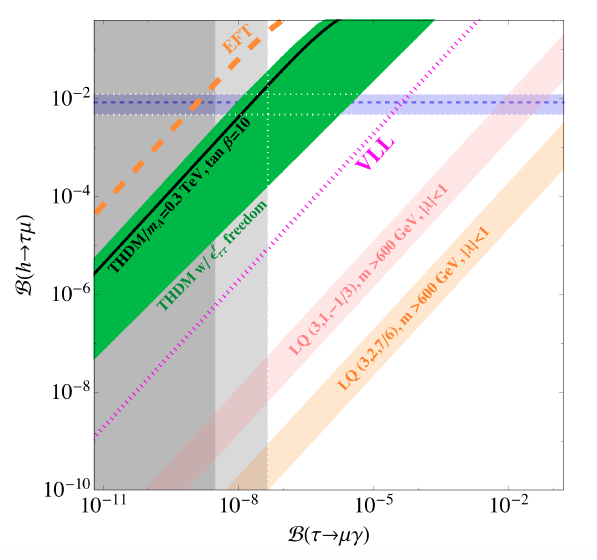
\includegraphics[width=0.7\textwidth]{images/h-vs-tau.png}
\caption{Correlation between $\br(\htm)$ and $\br(\tmg)$ in various NP scenarios (Dorsner et al., 2015)}
\label{}
\end{figure}


The present experimental result for $\br(\htm)$ is shown in horizontal blue band; current and future projections for $\br(\tmg)$ experimental sensitivity are represented with vertical light and dark gray bands. We note that certain 2HDM models predict a branching fraction for $\br(\tmg)$, consistent with the CMS results, at sensitivities which could be observed by Belle II. It is important to note that the Higgs sector could contribute to LFV in NP scenarios, and that both theory and experimental limits on other LFV processes such as $\htm$ all interweave with limits on $\tlg$ branching fractions to provide information on NP, even just through reducing the available phase space for certain models \cite{Dorsner:2015}.

\begin{figure}[h]
\centering
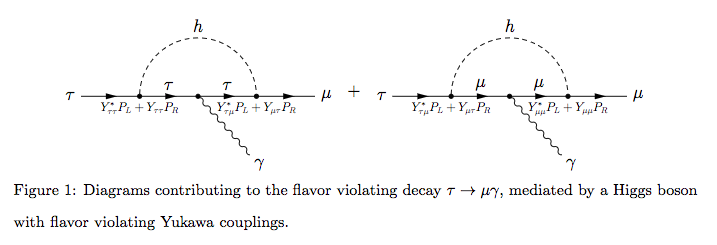
\includegraphics[width=0.9\textwidth]{images/higgs-lfv-modes.png}
\caption{Diagrams contributing to $\tmg$ decay, mediated by a Higgs boson with flavour violating Yukawa coupling (Harnick et al., 2012)}
\label{}
\end{figure}

As seen in Figure above, new Higgs particles can mediate LFV processes and allow for measurable amounts of LFV beyond the Standard Model \cite{Dorsner:2015}.


\subsubsection{Models predicting $\tlg$}

As mentioned previously, LFV in the $\tau$ sector is introduced in many NP scenarios as a consequence of generating neutrino mass (and hence facilitating neutrino mixing). Branching fractions of the modes $\tlg$ are highly calculable - there is little theoretical uncertainty.

\begin{figure}[h]
\centering
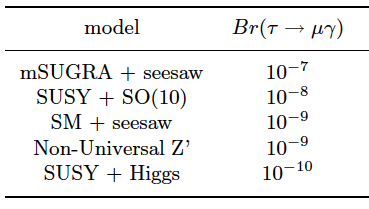
\includegraphics[width=0.5\textwidth]{images/np-models-bounds.png}
\caption{Upper limits of branching fractions from $\tmg$, predicted by models of new physics beyond the SM (various sources)\cite{Ohshima:2007zz}}
\label{}
\end{figure}

Figure above lists a few NP models with their predictions of $\br(\tmg)$. We see that the phase space of some of these models has already been ruled out with our current experimental limits on LFV branching fractions.



\subsection{Searches for $\tlg$}

The most recent searches for $\tlg$ were undertaken at Belle (2007) and Babar (2010), for both $\ell=\mu,e$ modes. These detectors are $e^+ e^-$ colliders; a signal of the form $e^+ e^-\to \tau^+ \tau^-$, with one tau (signal-side) decaying $\tau\to \ell \gamma$ and the other tau (tag-side) decaying generically, with the requirement that the tag-side track is not $\ell$.

The dominant backgrounds for the process $\tmg$ are $\tau\to \mu \nu \nu$, $\tau\to \pi \nu$ and $e^+ e^- \to \mu^+ \mu^- \gamma$ (with similar backgrounds for $\tau\to e \gamma$) \cite{Hayasaka:2007}. The first two backgrounds have branching fractions
\begin{align}
\br(\tau\to \mu \nu \nu)&=17.41\%\\
\br(\tau\to\pi\nu)&=10.83\%
\end{align}
which are non-negligible contributions to the dataset. The cross-section for we can compare the cross section of $e^+ e^- \to \mu^+ \mu^- \gamma$ to that of $e^+ e^- \to \tau^+ \tau^- \gamma$;
\begin{align}
\sigma(e^+ e^- \to \mu^+ \mu^- \gamma)&=\SI{0.242}{nb}\\
\sigma(e^+ e^- \to \tau^+ \tau^- \gamma)&=\SI{0.919}{nb}\\
\end{align}
so we note a significant contribution from this background also.

\begin{figure}[h]
\centering
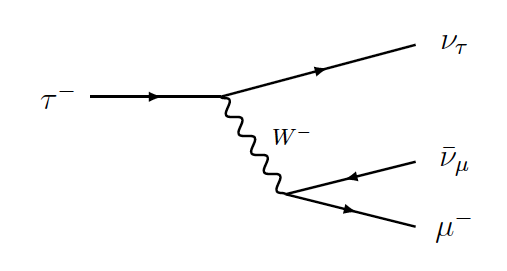
\includegraphics[width=0.3\textwidth]{images/taumununu.png}
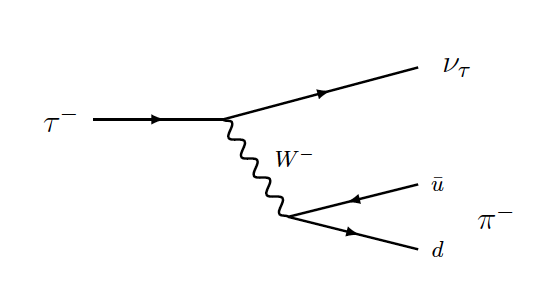
\includegraphics[width=0.3\textwidth]{images/taupinu.png}
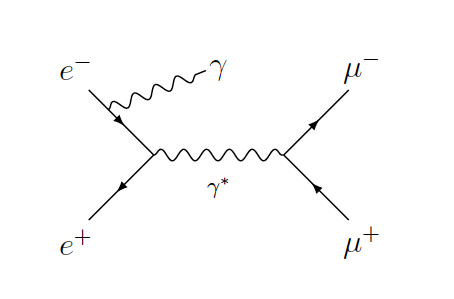
\includegraphics[width=0.3\textwidth]{images/eemumugamma.png}
\caption{Dominant backgrounds to $\tmg$. From left-to-right: $\tau\to \mu \nu \nu$, $\tau\to \pi \nu$ and $e^+ e^- \to \mu^+ \mu^- \gamma$}
\end{figure}


\subsubsection{Belle searches}


The Belle detector records events from an asymmetric $e^+ e^-$ collider with electron (positron) energy of $\SI{8}{GeV}$ ($\SI{3.5}{GeV}$). A detailed discussion of the detector can be found at Ref. \cite{Belle:2002}. In 2007, the Belle Collaboration performed a search over $\SI{535}{fb^{-1}}$ of $e^+ e^-$ data and set constraints \cite{Hayasaka:2007} on $\tlg$ branching fractions as

\begin{align}
\br(\tmg)&<\SI{4.5d-8}{}\\
\br(\tau\to e \gamma)&<\SI{1.2d-7}{}
\end{align}


\subsubsection{Babar searches}

Similar to Belle, the Babar detector records events from an asymmetric $e^+e^-$ collider, with electron (positron) energy of $\SI{9}{GeV}$ ($\SI{3.1}{GeV}$). A detailed discussion of the detector can be found at Ref. \cite{Babar:2002}. The most recent search for $\tlg$ was performed in 2010 by the Babar Collaboration \cite{Babar:2010}, over a $\SI{515.5}{fb^{-1}}$ dataset, setting constraints on $\tlg$ branching fractions as

\begin{align}
\br(\tmg)&<\SI{4.4d-8}{}\\
\br(\tau\to e \gamma)&<\SI{3.3d-8}{}
\end{align}



\subsection{Future searches}

\subsubsection{Belle II}

To probe smaller branching fractions for signals of new physics, we are required to build particle detectors with greater total integrated luminosity. The Belle II experiment, the successor to the Belle experiment, has a predicted total integrated luminosity of $\SI{50}{ab^{-1}}$. As a point of comparison, the Belle experiment collected $\SI{1000}{fb^{-1}}$ of data over its lifetime. A detailed discussion on the Belle II detector can be found at Ref \cite{Belle:2010}.

\begin{figure}[h]
\centering
%\includegraphics[width=0.9\textwidth]{images/tauLFV.png}
\caption{Current and future sensitivities on $\tau$ LFV branching fractions (Urquijo, 2016)}
\end{figure}

Increased luminosity will allow the branching fractions of various LFV processes to be probed with greater sensitivity. Figure above gives an indication of how future searches at Belle II will improve upper limits on the branching fractions for decays such as, importantly, $\tlg$.



%-------------------------------------------------------------------


\section{The Belle and Belle II detectors}

Located at 36° 9′ 17″ N, 140° 4′ 19″ E, or {36.154722, 140.071944}, is the KEKB particle accelerator. This accelerator was used for the Belle experiment from ???? to ???? and collided high energy electrons and positrons of $\SI{8}{GeV}$ and $\SI{3.5}{GeV}$ respectively. Over its lifetime, the Belle detector collected a total integrated luminosity of $\SI{1000}{fb-1}$, corresponding to ???? tau-pair events (from which our signal mode could occur).

The key components of the detector are the silicon vertex detector (SVD), the central drift chamber (CDC), electromagnetic calorimeter (ECL), time-of-flight/Cerenkov aerogel chamber (TOP), and the K-long/muon detector (KLM).

%-------------------------------------------------------------------


\subsection{	Silicon Vertex Detector}


%-------------------------------------------------------------------


\subsection{	Central Drift Chamber}

%-------------------------------------------------------------------


\subsection{Electromagnetic Calorimeter}

%-------------------------------------------------------------------


\subsection{Time-of-flight/Cerenkov aerogel chamber}

%-------------------------------------------------------------------


\subsection{K-long/muon detector}


%-------------------------------------------------------------------



\subsection{Super-KEKB upgrades/differences}


%-------------------------------------------------------------------


\section{Monte Carlo production and background types}

%-------------------------------------------------------------------


\section{Reconstruction and pre-selection}



%-------------------------------------------------------------------

\section{Correlation}



%-------------------------------------------------------------------

\section{Scalings and signal optimisation}


%-------------------------------------------------------------------

\section{Signal region and event selection}


\section{Conclusion}

\lipsum[1]



%-----------------------------------------
\bibliographystyle{plain}
\bibliography{refs.bib}
\end{document}







